\section{实现与收敛}
\label{sec:block-implementation}

前面几节给出了更新公式。本节把它们放回实际运行的环境，回答：更新怎样读值，内层要解到多准，算法能保证什么，总计算量是否真的省了？下面的结论都与具体的选块规则、模型条件和误差要求绑定，评价进展时统一看完整目标。

\subsection{串行与并行}
\label{sec:block-parallel}

\paragraph{串行读新值，并行读旧值}
串行时，每一块读取的都是已经更新过的最新值。并行时，多块基于同一个旧点同时计算，然后同时写入。这看起来只差一点，实际上改变了算法的性质：串行步长的保证建立在“只有一块变化”上，而并行时变化的是几块的和。

用最小的例子看。目标是
\[
 f(u,v)=\frac12(u+v)^2,\qquad (u,v)=(1,1).
\]
每个坐标的块光滑常数都是$1$。串行时，先更新$u$，得$u=1-2=-1$，到达$(-1,1)$，目标值$0$，已经最优。

并行时，两个坐标都读$u+v=2$，都走同样的一步，得到
\[
 (u,v)=(1,1)-(2,2)=(-1,-1),
\]
目标值仍是$2$。下一步又回到$(1,1)$，迭代在这两点之间振荡，永远不动。每一块单独都沿下降方向走，合起来却越过了最低点。图~\ref{fig:block-parallel-jacobi}(a)是这条路径。

\paragraph{覆盖同时变化的联合上界}
上界~\eqref{eq:block-quadratic-upper}只对一块变化成立。要保证并行步，需要一个覆盖几块同时变化的上界。下面的引理说明，对凸目标，只需把步长缩小到同时更新块数的倒数。

\begin{lemma}[并行更新的联合上界]
\label{lem:block-parallel-upper}
设$f$是凸函数，且满足定义~\ref{def:block-smooth}。$\mathcal{S}$是含$\tau$个块的集合，$\bm{h}_J\in\mathbb{R}^{\lvert J\rvert}$（$J\in\mathcal{S}$）。则
\begin{equation}
 f\Bigl(\bm{x}+\sum_{J\in\mathcal{S}}\bm{U}_J\bm{h}_J\Bigr)
 \leq f(\bm{x})+\sum_{J\in\mathcal{S}}\langle\nabla_Jf(\bm{x}),\bm{h}_J\rangle+\frac{\tau}{2}\sum_{J\in\mathcal{S}}L_J\lVert\bm{h}_J\rVert_2^2 .
 \label{eq:block-parallel-upper}
\end{equation}
\end{lemma}

\begin{proof}
把位移写成$\tau$个块方向的平均：
\[
 \bm{x}+\sum_{J\in\mathcal{S}}\bm{U}_J\bm{h}_J=\frac{1}{\tau}\sum_{J\in\mathcal{S}}\bigl(\bm{x}+\tau\bm{U}_J\bm{h}_J\bigr).
\]

由$f$的凸性，
\[
 f\Bigl(\bm{x}+\sum_{J\in\mathcal{S}}\bm{U}_J\bm{h}_J\Bigr)\leq\frac{1}{\tau}\sum_{J\in\mathcal{S}}f\bigl(\bm{x}+\tau\bm{U}_J\bm{h}_J\bigr).
\]

对每一项用上界~\eqref{eq:block-quadratic-upper}，位移取$\tau\bm{h}_J$：
\[
 f\bigl(\bm{x}+\tau\bm{U}_J\bm{h}_J\bigr)\leq f(\bm{x})+\tau\langle\nabla_Jf(\bm{x}),\bm{h}_J\rangle+\frac{L_J\tau^2}{2}\lVert\bm{h}_J\rVert_2^2 .
\]
代入后除以$\tau$，即得式~\eqref{eq:block-parallel-upper}。
\end{proof}

式~\eqref{eq:block-parallel-upper}的右边对各块可分，分别最小化，得到每块的并行步长$1/(\tau L_J)$，并且保证下降量至少是
\begin{equation}
 \frac{1}{2\tau}\sum_{J\in\mathcal{S}}\frac{\lVert\nabla_Jf(\bm{x})\rVert_2^2}{L_J} .
 \label{eq:block-parallel-decrease}
\end{equation}
例中$\tau=2$，步长是$\tfrac12$，两个坐标都走$-1$，一步到$(0,0)$。

这个因子$\tau$偏保守。对最小二乘，若$\bm{A}$的每一行最多有$\omega$个非零元，由Cauchy--Schwarz不等式，第$i$行满足
\[
 \Bigl(\sum_ja_{i,j}h_j\Bigr)^2\leq\omega\sum_ja_{i,j}^2h_j^2 .
\]
对所有行求和，二次项不超过$\omega\sum_jL_jh_j^2$，所以因子可以取$\min\{\tau,\omega\}$。变量之间的耦合越稀疏，并行越接近串行的效率。例中$\bm{A}$的第一行有两个非零元，$\omega=2$。

图~\ref{fig:block-parallel-jacobi}(b)是三变量的例子，$\bm{Q}=0.25\,\bm{I}+0.75\,\bm{1}\bm{1}^\top$。串行步长$\alpha=1$（$L_j=1$）用于并行时目标值发散，缩小到$\alpha=\tfrac13$后单调下降，但慢于串行。

\begin{BookInlineFigure}
  \centering
  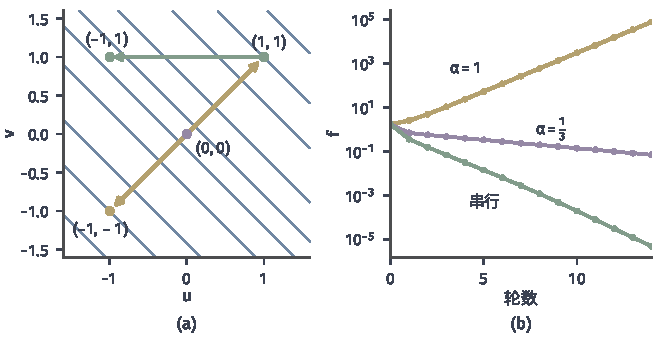
\includegraphics[width=112mm]{figures/05-optimization/04-block-optimization/matplotlib/block-parallel-jacobi/figure.pdf}
  \caption{串行与并行。(a)$f=\tfrac12(u+v)^2$从$(1,1)$出发：绿色是串行一步到达$(-1,1)$；黄色是并行且步长$1$，在$(1,1)$与$(-1,-1)$间振荡；紫点是并行且步长$\tfrac12$的结果$(0,0)$。(b)$n=3$、$\bm{Q}=0.25\,\bm{I}+0.75\,\bm{1}\bm{1}^\top$时目标值随轮数的变化：黄线是并行且步长$1$，紫线是并行且步长$\tfrac13$，绿线是串行且步长$1$。}
  \label{fig:block-parallel-jacobi}
\end{BookInlineFigure}

\paragraph{实现条件}
同步并行要在每轮末等所有块写完，这一等待有实际的时间成本。共享残差时，多个块同时写$\bm{r}$要处理写冲突；块的数据不重叠时才能完全并行。若不做同步，块会读到别的块更新到一半的旧值，这时上面的引理不再适用，需要另外分析读取延迟。

\subsection{子问题的求解精度}
\label{sec:block-inexact}

\paragraph{把误差计入下降量}
块子问题常常只能迭代求解。设$m$是当前块的模型（精确BCD时就是条件函数），$\bm{z}^\star$是模型的最小点。近似解$\tilde{\bm{z}}$的模型值误差为
\begin{equation}
 m(\tilde{\bm{z}})\leq m(\bm{z}^\star)+\varepsilon .
 \label{eq:block-inexact}
\end{equation}
若$m$是块上界，由上界与相等条件，近似解带来的完整目标下降至少是
\begin{equation}
 F(\bm{x})-F(\bm{x}^{+})\geq\bigl(m(\bm{x}_J)-m(\bm{z}^\star)\bigr)-\varepsilon .
 \label{eq:block-inexact-descent}
\end{equation}
也就是精确解的模型下降量，减去误差。

\paragraph{两种接受条件}
区分两种条件。“不劣于当前点”即$m(\tilde{\bm{z}})\leq m(\bm{x}_J)$，它能维持单调性，但太弱：$\tilde{\bm{z}}=\bm{x}_J$也能通过，一点进展都没有。

支持长期进展的是相对精度：取$0\leq\eta<1$，要求
\begin{equation}
 m(\tilde{\bm{z}})-m(\bm{z}^\star)\leq\eta\bigl(m(\bm{x}_J)-m(\bm{z}^\star)\bigr).
 \label{eq:block-relative-accuracy}
\end{equation}
由式~\eqref{eq:block-inexact-descent}，这样的近似解保留精确解模型下降量的$(1-\eta)$倍。精确解的所有保底下降界乘以$(1-\eta)$仍然成立，收敛速率只差一个常数因子。

\paragraph{怎样测量误差}
$m(\bm{z}^\star)$通常不知道，需要可计算的上界。设子问题是正定二次函数，$\bm{P}$是对称正定矩阵，且$\bm{P}\succeq\sigma\bm{I}$，$\sigma>0$：
\[
 m(\bm{z})=\frac12\bm{z}^\top\bm{P}\bm{z}-\bm{q}^\top\bm{z}.
\]
梯度残差$\bm{s}=\bm{P}\tilde{\bm{z}}-\bm{q}$是可以计算的。由$\bm{z}^\star=\bm{P}^{-1}\bm{q}$，得$\tilde{\bm{z}}-\bm{z}^\star=\bm{P}^{-1}\bm{s}$。二次函数在最小点附近精确地展开为
\[
 m(\tilde{\bm{z}})-m(\bm{z}^\star)=\frac12(\tilde{\bm{z}}-\bm{z}^\star)^\top\bm{P}(\tilde{\bm{z}}-\bm{z}^\star)=\frac12\bm{s}^\top\bm{P}^{-1}\bm{s}.
\]

再由$\bm{P}^{-1}$的最大特征值不超过$1/\sigma$，得到
\begin{equation}
 m(\tilde{\bm{z}})-m(\bm{z}^\star)\leq\frac{\lVert\bm{s}\rVert_2^2}{2\sigma}.
 \label{eq:block-residual-bound}
\end{equation}
例中$x_2=4$时，条件函数是$z^2+4z+16$，所以$P=2$，$q=-4$，$\sigma=2$。取$\tilde{z}=-1.9$，残差$s=2(-1.9)+4=0.2$，误差确实是$(-1.9+2)^2=0.01$，而界$s^2/(2\sigma)=0.04/4=0.01$恰好取到。

\paragraph{固定绝对误差的精度限制}
若每步都有相同的绝对误差$\varepsilon$，长期结果就有下限。设无误差时有收缩$E^{(t+1)}\leq(1-\rho)E^{(t)}$，$0<\rho<1$，这里$E^{(t)}$是目标差或其期望。由式~\eqref{eq:block-inexact-descent}，有误差时变成
\[
 E^{(t+1)}\leq(1-\rho)E^{(t)}+\varepsilon .
\]
展开这个递推，并对等比级数求和，得到
\begin{equation}
 E^{(T)}\leq(1-\rho)^TE^{(0)}+\frac{\varepsilon}{\rho}.
 \label{eq:block-error-floor}
\end{equation}
第一项趋于零，第二项不会消失，算法最终停在一个与$\varepsilon/\rho$同量级的平台上。图~\ref{fig:block-inexact-accuracy}的黄线就是这个平台，紫线用相对精度~\eqref{eq:block-relative-accuracy}的同类要求，一直下降，只是比精确解慢一些。

\begin{BookInlineFigure}
  \centering
  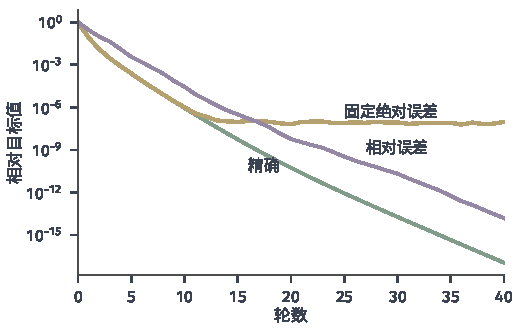
\includegraphics[width=88mm]{figures/05-optimization/04-block-optimization/matplotlib/block-inexact-accuracy/figure.pdf}
  \caption{块子问题误差的影响。$n=40$的正定二次目标，每块$8$个变量，循环更新。绿线是精确块解；黄线的每次块解有固定的残差范数$10^{-3}$，目标值停在平台上；紫线的残差范数取当前偏梯度范数的一半，仍线性收敛。}
  \label{fig:block-inexact-accuracy}
\end{BookInlineFigure}

\paragraph{内层成本与解的复用}
相对精度也有成本。把一块解到较高精度需要更多内层迭代，而上一轮的块解是内层求解的好起点，这称为热启动；固定曲率时，矩阵分解还能重复使用。接受标准定得太严，一步就要做很多无用的内层迭代；定得太松，外层要多走好多轮。两者的总和才是要比较的量。

\subsection{收敛保证}
\label{sec:block-convergence}

\paragraph{三个不同的问题}
“算法收敛”可以指三件不同的事，由弱到强依次是：目标值序列收敛；迭代点的聚点是驻点；整个迭代点序列收敛到一点。下面分别看各需要什么条件。

\paragraph{目标值收敛}
只要每步不增且目标有下界，目标值序列就收敛。精确块更新由引理~\ref{lem:block-exact-descent}满足单调性，BCGD由式~\eqref{eq:block-bcgd-decrease}满足，BSUM由式~\eqref{eq:block-bsum-descent}满足，BPG由式~\eqref{eq:block-prox-descent}满足。这个结论很弱，它不说明目标值收敛到哪里，更不说明点收敛。

\paragraph{聚点驻定}
聚点的性质需要逐条检查四件事：块访问，即每一块都被反复更新；解的选择，即子问题的解有确定的规则，这里要求唯一；水平集条件，使迭代有聚点；以及分块的最优性条件能否合成整体驻点条件。

下面给出循环规则下的结论。设$\bm{C}$是闭凸集的乘积，$F$在$\bm{C}$上连续。

\begin{theorem}[循环BSUM的聚点]
\label{thm:block-bsum-limit}
设$\bm{x}^{(0)}\in\bm{C}$，下水平集
\begin{equation}
 \bm{S}=\{\bm{x}\in\bm{C}:F(\bm{x})\leq F(\bm{x}^{(0)})\}
 \label{eq:block-level-set}
\end{equation}
是紧集。设每个块的$u_J$满足定义~\ref{def:block-upper-bound}，且对每个$\bm{y}\in\bm{S}$，$u_J(\cdot;\bm{y})$在$\bm{C}_J$上有唯一的最小点。按固定顺序循环更新各块，则每轮开始时的点列$\{\bm{x}^{(t)}\}$有聚点，并且每个聚点$\bar{\bm{x}}$满足
\begin{equation}
 \bar{\bm{x}}_J=\argmin_{\bm{z}\in\bm{C}_J}u_J(\bm{z};\bar{\bm{x}})\quad\text{对每个块}\ J,
 \label{eq:block-limit-fixed}
\end{equation}
\begin{equation}
 F'(\bar{\bm{x}};\bm{U}_J\bm{d})\geq0\quad\text{对每个块}\ J\ \text{和满足}\ \bar{\bm{x}}_J+\bm{d}\in\bm{C}_J\ \text{的}\ \bm{d}.
 \label{eq:block-limit-directional}
\end{equation}
\end{theorem}

\begin{proof}
记$M_J(\bm{y})$为只把$\bm{y}$的块$J$替换成$u_J(\cdot;\bm{y})$的最小点得到的点。由下降链~\eqref{eq:block-bsum-descent}，$M_J$把$\bm{S}$映入$\bm{S}$，迭代始终留在$\bm{S}$中。$\bm{S}$紧，所以聚点存在，$F(\bm{x}^{(t)})$单调有界而收敛到某个$\bar{F}$，由连续性，每个聚点满足$F(\bar{\bm{x}})=\bar{F}$。

先证$M_J$在$\bm{S}$上连续。设$\bm{y}^{(k)}\to\bm{y}$，$\bm{y}^{(k)}\in\bm{S}$，任取$M_J(\bm{y}^{(k)})$的一个收敛子列，极限$\bar{\bm{z}}$在$\bm{S}$中，且只在块$J$上与$\bm{y}$不同。对任意$\bm{w}\in\bm{C}_J$，有
\[
 u_J\bigl(M_J(\bm{y}^{(k)})_J;\bm{y}^{(k)}\bigr)\leq u_J(\bm{w};\bm{y}^{(k)}).
\]
令$k\to\infty$，由$u_J$的连续性，$\bar{\bm{z}}_J$是$u_J(\cdot;\bm{y})$的最小点，由唯一性，$\bar{\bm{z}}=M_J(\bm{y})$。紧集中的序列每个收敛子列的极限都相同，所以$M_J(\bm{y}^{(k)})\to M_J(\bm{y})$。

再设子列$\bm{x}^{(t_j)}\to\bar{\bm{x}}$，块的顺序是$J_1,\ldots,J_B$。令$\bm{z}^{j,0}=\bm{x}^{(t_j)}$，$\bm{z}^{j,k}=M_{J_k}(\bm{z}^{j,k-1})$。下面对$k$归纳证明$\bm{z}^{j,k}\to\bar{\bm{x}}$（$j\to\infty$）。设$\bm{z}^{j,k-1}\to\bar{\bm{x}}$，由$M_{J_k}$的连续性，$\bm{z}^{j,k}$收敛到点
\[
 \bar{\bm{w}}=M_{J_k}(\bar{\bm{x}}).
\]

由单调性，
\[
 F(\bm{x}^{(t_j+1)})\leq F(\bm{z}^{j,k})\leq F(\bm{x}^{(t_j)}),
\]
两端都趋于$\bar{F}$，所以$F(\bar{\bm{w}})=\bar{F}$。再由下降链，
\[
 \bar{F}=F(\bar{\bm{w}})\leq u_{J_k}(\bar{\bm{w}}_{J_k};\bar{\bm{x}})\leq u_{J_k}(\bar{\bm{x}}_{J_k};\bar{\bm{x}})=F(\bar{\bm{x}})=\bar{F}.
\]
这表明$\bar{\bm{x}}_{J_k}$也是$u_{J_k}(\cdot;\bar{\bm{x}})$的最小点。由唯一性，$\bar{\bm{w}}=\bar{\bm{x}}$，归纳完成，并且式~\eqref{eq:block-limit-fixed}对每个$J_k$成立。

最后，$\bar{\bm{x}}_J$最小化$u_J(\cdot;\bar{\bm{x}})$，$\bm{C}_J$是凸集，所以沿任何可行方向的方向导数非负。由一阶条件~\eqref{eq:block-ub-derivative}，这就是式~\eqref{eq:block-limit-directional}。
\end{proof}

取$u_J$为条件函数，定理就覆盖了精确BCD。定理中的条件各有用处：紧性让聚点存在；唯一性决定了不动点论证中的$\bar{\bm{w}}=\bar{\bm{x}}$；循环访问保证每个块都被访问到。“每隔固定步数每块至少访问一次”的规则也能用同样的论证。

\paragraph{唯一性去掉会怎样}
最小点不唯一时，聚点可以不是驻点。一个经典的三变量例子是
\[
 f(\bm{x})=-(x_1x_2+x_2x_3+x_3x_1)+\sum_{i=1}^{3}(\lvert x_i\rvert-1)_+^2 ,
\]
其中$(s)_+=\max\{s,0\}$。固定其余两个变量，令和为$s\neq0$时，$x_1$的最小点唯一，是$\operatorname{sign}(s)(1+\lvert s\rvert/2)$；$s=0$时，$[-1,1]$上每一点都是最小点。

从下面的起点出发循环更新，$\epsilon>0$：
\[
 \bm{x}^{(0)}=\Bigl(-1-\epsilon,\ 1+\frac{\epsilon}{2},\ -1-\frac{\epsilon}{4}\Bigr).
\]
三步之后的三个坐标依次是
\[
 x_1=1+\frac{\epsilon}{8},\qquad x_2=-1-\frac{\epsilon}{16},\qquad x_3=1+\frac{\epsilon}{32}.
\]
每次偏离$\pm1$的量缩小到一半，符号不断翻转，迭代点沿立方体的六个顶点循环，聚点是这些顶点。

顶点不是驻点，比如$(1,1,-1)$处$\partial_3f=-2$，$\partial_1f=\partial_2f=0$。问题正出在极限处$s=0$：条件子问题的最小点不再唯一，$M_J$不再连续，定理的论证在这里断开。这个例子的目标也没有下界，这里关心的是解的选择造成的现象，水平集条件并不是它失效的主因。

\paragraph{合成整体驻点}
式~\eqref{eq:block-limit-directional}只说沿块方向的方向导数非负。能否合成整体驻点，要看方向导数在块间是否可加。$F$可微时，方向导数按块相加：
\[
 F'(\bar{\bm{x}};\bm{d})=\sum_J\langle\nabla_JF(\bar{\bm{x}}),\bm{d}_J\rangle ,
\]
每一项非负，和也非负，这就是闭凸可行域上的驻点条件。

$F=f+\sum_Jg_J$且$g_J$凸时，方向导数同样按块相加，结论也成立；$F$凸时由此得到全局最优。例~\eqref{eq:block-nonsmooth-example}的方向导数不能按块分开，这一步失败。

\paragraph{整列收敛}
聚点驻定仍然允许序列在几个驻点之间徘徊。整列收敛到一点需要更强的条件，典型的是强凸性。若$F$是$\mu$强凸的且$F(\bm{x}^{(t)})\to F^\star$，则由
\[
 \frac{\mu}{2}\lVert\bm{x}^{(t)}-\bm{x}^\star\rVert_2^2\leq F(\bm{x}^{(t)})-F^\star
\]
得到$\bm{x}^{(t)}\to\bm{x}^\star$。非强凸时需要借助目标在解附近的增长性质，这超出本章范围。

\paragraph{随机BCGD的有限步界}
上面的结论都是渐近的，下面给出有限步的结果。这里考虑独立均匀选块、使用精确偏梯度的BCGD，分析的关键仍是单步的平均下降。

\begin{theorem}[随机BCGD的收敛率]
\label{thm:block-rbcgd}
设$f:\mathbb{R}^n\to\mathbb{R}$有下界$f^\star$，关于每一块是$L_J$光滑的，记$L_{\max}=\max_JL_J$。每步与历史独立地均匀抽取一块，按式~\eqref{eq:block-bcgd}更新。则有
\begin{equation}
 \mathbb{E}\bigl[f(\bm{x}^{(t+1)})\mid\bm{x}^{(t)}\bigr]\leq f(\bm{x}^{(t)})-\frac{1}{2BL_{\max}}\lVert\nabla f(\bm{x}^{(t)})\rVert_2^2 ,
 \label{eq:block-rbcgd-one-step}
\end{equation}
\begin{equation}
 \min_{0\leq t<T}\mathbb{E}\lVert\nabla f(\bm{x}^{(t)})\rVert_2^2\leq\frac{2BL_{\max}\bigl(f(\bm{x}^{(0)})-f^\star\bigr)}{T}.
 \label{eq:block-rbcgd-gradient}
\end{equation}
若$f$还是$\mu$强凸的，则
\begin{equation}
 \mathbb{E}f(\bm{x}^{(T)})-f^\star\leq\Bigl(1-\frac{\mu}{BL_{\max}}\Bigr)^{T}\bigl(f(\bm{x}^{(0)})-f^\star\bigr).
 \label{eq:block-rbcgd-linear}
\end{equation}
\end{theorem}

\begin{proof}
抽到块$J$的概率是$1/B$，由式~\eqref{eq:block-bcgd-decrease}，此时下降量至少是$\lVert\nabla_Jf\rVert_2^2/(2L_J)$。对$B$个块取平均，并用$L_J\leq L_{\max}$，得到
\[
 \mathbb{E}\bigl[f(\bm{x}^{(t+1)})\mid\bm{x}^{(t)}\bigr]\leq f(\bm{x}^{(t)})-\frac{1}{2BL_{\max}}\sum_J\lVert\nabla_Jf(\bm{x}^{(t)})\rVert_2^2 .
\]
各块的下标互不重叠且并起来是全部下标，所以
\[
 \sum_J\lVert\nabla_Jf\rVert_2^2=\lVert\nabla f\rVert_2^2 ,
\]
这就是式~\eqref{eq:block-rbcgd-one-step}。

对式~\eqref{eq:block-rbcgd-one-step}取全期望，并对$t=0,\ldots,T-1$求和，左右两边的目标值相消，得到
\[
 \frac{1}{2BL_{\max}}\sum_{t=0}^{T-1}\mathbb{E}\lVert\nabla f(\bm{x}^{(t)})\rVert_2^2\leq f(\bm{x}^{(0)})-\mathbb{E}f(\bm{x}^{(T)})\leq f(\bm{x}^{(0)})-f^\star .
\]
最小值不超过平均值，移项即得式~\eqref{eq:block-rbcgd-gradient}。

强凸时，把强凸下界对$\bm{y}$取最小：
\[
 \begin{aligned}
 f^\star&\geq\min_{\bm{y}}\Bigl\{f(\bm{x})+\langle\nabla f(\bm{x}),\bm{y}-\bm{x}\rangle+\frac{\mu}{2}\lVert\bm{y}-\bm{x}\rVert_2^2\Bigr\}\\
 &=f(\bm{x})-\frac{1}{2\mu}\lVert\nabla f(\bm{x})\rVert_2^2 ,
 \end{aligned}
\]
也就是
\[
 \lVert\nabla f(\bm{x})\rVert_2^2\geq2\mu\bigl(f(\bm{x})-f^\star\bigr).
\]
把它代入式~\eqref{eq:block-rbcgd-one-step}，两边减去$f^\star$，得到
\[
 \mathbb{E}\bigl[f(\bm{x}^{(t+1)})-f^\star\mid\bm{x}^{(t)}\bigr]\leq\Bigl(1-\frac{\mu}{BL_{\max}}\Bigr)\bigl(f(\bm{x}^{(t)})-f^\star\bigr).
\]
取全期望并反复使用即得式~\eqref{eq:block-rbcgd-linear}。
\end{proof}

例中$B=2$，$L_{\max}=2$，$\mu=1$，因子是$\tfrac34$。从$f=37$出发一步后，定理的上界是$27.75$，实际的平均值是$9.375$：定理只用了最坏的块光滑常数，实际情况好得多。

$B$次更新的成本约等于一次全梯度，这时因子约为$1-\mu/L_{\max}$。与第~\ref{chap:first-order-methods}章梯度下降每步的$1-\mu/L$相比，$L_{\max}$越小于$L$，块方法越有优势\scite{nesterov2012efficiency}。式~\eqref{eq:block-constant-order}中的$L_j\leq L$保证了这个比较不会反过来。

\paragraph{加速方法另当别论}
定理~\ref{thm:block-rbcgd}的论证依赖于每步的单调下降。APCG的$F(\bm{x}^{(t)})$不是单调的，这里的论证用不上，定理~\ref{thm:block-apcg}的结论要靠辅助序列的递推才能得到。

\subsection{计算成本}
\label{sec:block-cost}

\paragraph{一次更新的读取量}
最后回到开头的问题：计算真的省了吗？以稠密的$\bm{A}\in\mathbb{R}^{N\times n}$为例，比较三种操作的运算量（只数乘法）。一次单坐标更新要读$\bm{a}_j^\top\bm{r}$和更新$\bm{r}$，各需$N$次；一次完整遍历$n$个坐标，一次全梯度要算$\bm{A}\bm{x}$和$\bm{A}^\top\bm{r}$，结果如下表。

\begin{BookInlineTable}
\centering
\begin{tabular}{lll}
\toprule
操作 & 稠密$\bm{A}$ & 稀疏$\bm{A}$\\
\midrule
一次单坐标更新 & $2N$ & $2\operatorname{nnz}(\bm{a}_j)$\\
一轮（$n$次更新） & $2Nn$ & $2\operatorname{nnz}(\bm{A})$\\
一次全梯度 & $2Nn$ & $2\operatorname{nnz}(\bm{A})$\\
\bottomrule
\end{tabular}
\end{BookInlineTable}

由此可知，维护残差之后，一轮坐标更新和一次全梯度的成本相同。若没有维护残差，每次更新都重算$\bm{A}\bm{x}$，一轮的成本就变成全梯度的$n$倍，优势全失。

例中$\bm{A}$每列两个非零元，一次更新要$4$次乘法，一轮$8$次，一次全梯度也是$8$次。花同样的计算，一轮循环坐标下降把目标值乘以$\tfrac{1}{16}$，最优固定步长的梯度下降每步只乘以$\tfrac14$（$\kappa=3$，由第~\ref{chap:first-order-methods}章的结论，$((\kappa-1)/(\kappa+1))^2=\tfrac14$）。

\paragraph{完整的成本清单}
比较几种方法要用同一个目标和同一个精度要求，并把下表中的所有项计入，只算迭代次数或只算单步代价都会得出错误的结论。

\begin{BookInlineTable}
\centering
\begin{tabular}{p{14mm}p{42mm}p{36mm}}
\toprule
项目 & 何时发生 & 怎样减少\\
\midrule
选块 & 贪心规则要所有块的偏梯度 & 增量维护、优先队列\\
曲率形成 & 块Newton、$L_J$的计算 & 只算一次、用上界估计\\
内层求解 & 精确块解、块Newton、$\bm{U}$的方程 & 复用分解、热启动\\
外推 & APCG的全向量组合 & 用两个基向量表示\\
内存 & 残差、偏梯度、分解因子 & 只保留必要的中间量\\
同步 & 并行时的等待与写冲突 & 块之间数据不重叠\\
\bottomrule
\end{tabular}
\end{BookInlineTable}

检查“较少的块更新是否真正减少总工作量”时，要回到图~\ref{fig:block-size-cost}(b)的做法：把横轴换成总运算量。块大一倍、轮数减半不一定划算，贪心规则迭代次数少也不一定划算；只有总运算量下降，才算真正的进步。
